\documentclass[11pt]{article}

\usepackage[a4paper]{geometry}
\geometry{left=2.0cm,right=2.0cm,top=3cm,bottom=2.5cm}
\usepackage{setspace}
\setstretch{1.5}
\usepackage{ctex}
\usepackage{amsmath,amsfonts,graphicx,amssymb,bm,amsthm}
\usepackage{algorithm,algorithmicx}
\usepackage[noend]{algpseudocode}
\usepackage{fancyhdr}
\usepackage{booktabs}
\usepackage{array}
\usepackage{float}
\usepackage{listings}
\usepackage{xcolor}
\lstset{
	language=Python,
	basicstyle=\ttfamily\small,
	numbers=left,
	numberstyle=\tiny\color{teal!70!black},
	showstringspaces=false,
	breaklines=true,
	frame=single,
	rulecolor=\color{black},
	framerule=0.6pt,
	framesep=4pt,
	xleftmargin=6pt,
	backgroundcolor=\color{gray!4},
	columns=fullflexible,
	keywordstyle=\bfseries\color{blue!70!black},
	commentstyle=\itshape\color{green!50!black},
	stringstyle=\color{red!60!black},
	identifierstyle=\color{violet!70!black},
	emphstyle=\bfseries\color{orange!80!black},
	tabsize=4
}
\newcolumntype{M}[1]{>{\centering\arraybackslash}m{#1}}
\setlength{\headheight}{14pt}
\begin{document}
	\pagestyle{fancy}
	\lhead{\kaishu 中国科学院大学}
	\chead{}
	\rhead{\kaishu 2026年春季学期\qquad 深度学习}
	
	\begin{center}
		{\LARGE \bf 实验一：手写数字识别} 
	\end{center}
	\begin{center}
		\large\kaishu{尧祥临 202518023406038 前沿交叉科学学院}
	\end{center}

	\section{任务介绍}
	本次实验的任务是在MNIST手写数字数据集上构造并训练一个卷积神经网络模型，实现对0到9共10类手写数字图象的分类。实验指导书要求完成PyTorch环境搭建、MNIST数据加载、卷积神经网络组织结构构建、训练与评估，并使测试集准确率达到98\%及以上。

	MNIST数据集由灰度手写数字图象组成，每张图象大小为$28\times 28$。本实验中使用torchvision提供的数据接口加载数据，训练集原始规模为60000张，测试集规模为10000张。为了观察训练过程中的泛化表现，我将原始训练集划分为55000张训练样本和5000张验证样本，测试集保持为10000张样本。所有输入图象只进行\texttt{ToTensor}转换，没有额外使用数据增强操作。

	\section{模型架构}
	为了匹配MNIST图象分辨率较小、类别数较少的特点，本实验没有采用过深的网络，而是实现了一个由两组卷积、激活和池化层组成的CNN模型。整体流程为
	\[
		\begin{aligned}
			&\mathrm{Input}\rightarrow\mathrm{Conv2d}\rightarrow\mathrm{ReLU}\rightarrow\mathrm{MaxPool}\\
			&\rightarrow\mathrm{Conv2d}\rightarrow\mathrm{ReLU}\rightarrow\mathrm{MaxPool}\\
			&\rightarrow\mathrm{Flatten}\rightarrow\mathrm{Linear}\rightarrow\mathrm{ReLU}\rightarrow\mathrm{Linear}.
		\end{aligned}
	\]
	卷积层的输出尺寸可由下式计算：
	\[
		H_{\mathrm{out}}=\left\lfloor\frac{H_{\mathrm{in}}+2P-K}{S}\right\rfloor+1,
	\]
	其中$H_{\mathrm{in}}$表示输入尺寸，$K$表示卷积核大小，$P$表示padding大小，$S$表示步长。本模型两个卷积层均采用$5\times 5$卷积核、步长为1、padding为2，因此卷积操作本身保持特征图空间尺寸不变；随后通过$2\times 2$最大池化将空间尺寸减半。

	\begin{table}[H]
		\centering
		\caption{CNN模型结构}
		\begin{tabular}{M{3.2cm} M{3.2cm} M{3.2cm} M{4.8cm}}
			\toprule
			层 & 参数设置 & 输出尺寸 & 说明 \\
			\midrule
			Input & -- & $1\times 28\times 28$ & MNIST灰度图象 \\
			Conv1 & $1\rightarrow 32$, $5\times 5$ & $32\times 28\times 28$ & padding为2，保持分辨率 \\
			ReLU1 & -- & $32\times 28\times 28$ & 引入非线性表达能力 \\
			MaxPool1 & $2\times 2$, stride 2 & $32\times 14\times 14$ & 下采样并增强局部平移鲁棒性 \\
			Conv2 & $32\rightarrow 64$, $5\times 5$ & $64\times 14\times 14$ & 提取更高层次特征 \\
			ReLU2 & -- & $64\times 14\times 14$ & 非线性激活 \\
			MaxPool2 & $2\times 2$, stride 2 & $64\times 7\times 7$ & 第二次下采样 \\
			Flatten & -- & $3136$ & 将特征图展平成向量 \\
			Linear1 & $3136\rightarrow 128$ & $128$ & 全连接隐藏层 \\
			Linear2 & $128\rightarrow 10$ & $10$ & 输出10个类别的logits \\
			\bottomrule
		\end{tabular}
	\end{table}

	按照上述结构计算，模型总参数量为454922。其中第一层卷积参数量为$1\times 32\times 5\times 5+32=832$，第二层卷积参数量为$32\times 64\times 5\times 5+64=51264$，两个全连接层参数量分别为401536和1290。可以看出，主要参数集中在从$64\times 7\times 7$特征图到128维隐藏表示的第一个全连接层中。

	模型在代码中的核心定义如下：
	\begin{lstlisting}
class CNN(nn.Module):
    def __init__(self, hidden_dim=128):
        super(CNN, self).__init__()
        self.conv1 = nn.Conv2d(1, 32, kernel_size=5, stride=1, padding=2)
        self.relu1 = nn.ReLU()
        self.pool1 = nn.MaxPool2d(kernel_size=2, stride=2)

        self.conv2 = nn.Conv2d(32, 64, kernel_size=5, stride=1, padding=2)
        self.relu2 = nn.ReLU()
        self.pool2 = nn.MaxPool2d(kernel_size=2, stride=2)

        self.fc = nn.Sequential(
            nn.Flatten(),
            nn.Linear(64 * 7 * 7, hidden_dim),
            nn.ReLU(),
            nn.Linear(hidden_dim, 10)
        )

    def forward(self, x):
        x = self.pool1(self.relu1(self.conv1(x)))
        x = self.pool2(self.relu2(self.conv2(x)))
        return self.fc(x)
	\end{lstlisting}

	\section{参数设置}
	本实验使用交叉熵损失函数训练多分类模型。设单个batch大小为$B$，第$i$个样本对应类别为$y_i$，模型输出logits为$z_i$，则损失函数为
	\[
		\mathcal{L}=-\frac{1}{B}\sum_{i=1}^{B}
		\log \frac{\exp(z_{i,y_i})}{\sum_{c=0}^{9}\exp(z_{i,c})}.
	\]
	优化器采用AdamW。相比普通随机梯度下降，AdamW能够根据梯度一阶矩和二阶矩的估计自适应调整参数更新幅度，并将权重衰减与梯度更新解耦，对这种中小规模CNN训练较为稳定。具体超参数如表2所示。

	\begin{table}[H]
		\centering
		\caption{训练超参数设置}
		\begin{tabular}{M{4.5cm} M{7.5cm}}
			\toprule
			项目 & 设置 \\
			\midrule
			框架 & PyTorch, torchvision \\
			数据集 & MNIST, 训练/验证/测试划分为55000/5000/10000 \\
			输入预处理 & \texttt{transforms.ToTensor()} \\
			Batch size & 64 \\
			Epochs & 20 \\
			Learning rate & $5\times 10^{-4}$ \\
			隐藏层维度 & 128 \\
			损失函数 & \texttt{nn.CrossEntropyLoss()} \\
			优化器 & \texttt{torch.optim.AdamW} \\
			训练设备 & CUDA GPU \\
			模型保存路径 & \texttt{Lab1/model/cnn\_mnist.pth} \\
			日志保存路径 & \texttt{Lab1/logs/train\_log.csv} \\
			\bottomrule
		\end{tabular}
	\end{table}

	\section{训练过程}
	训练阶段，模型首先进入\texttt{train}模式，对每个batch执行前向传播、损失计算、反向传播和参数更新。验证与测试阶段，模型进入\texttt{eval}模式，并通过\texttt{torch.argmax}在10个输出logits中选取预测类别。训练过程中每个epoch结束后都会分别计算验证集和测试集上的loss与accuracy，并将结果写入CSV日志文件。

	\begin{lstlisting}
def train(model, train_loader, optimizer, criterion, device):
    model.train()
    total_loss = 0.0
    total_samples = 0
    for images, labels in train_loader:
        images, labels = images.to(device), labels.to(device)
        outputs = model(images)
        loss = criterion(outputs, labels)
        optimizer.zero_grad()
        loss.backward()
        optimizer.step()
        total_loss += loss.item() * images.size(0)
        total_samples += images.size(0)
    return total_loss / total_samples

def evaluate(model, data_loader, criterion, device):
    model.eval()
    correct = 0
    total = 0
    total_loss = 0.0
    for images, labels in data_loader:
        images, labels = images.to(device), labels.to(device)
        outputs = model(images)
        preds = torch.argmax(outputs, dim=1)
        loss = criterion(outputs, labels)
        total_loss += loss.item() * images.size(0)
        correct += (preds == labels).sum().item()
        total += labels.size(0)
    return total_loss / total, correct / total
	\end{lstlisting}

	表3给出了若干关键epoch的训练记录。可以看到，模型在第1个epoch结束时测试准确率已经达到98.32\%，超过实验要求的98\%；随着训练继续进行，训练损失持续下降，验证集和测试集准确率整体保持上升趋势，最终第20个epoch测试准确率达到99.33\%。

	\begin{table}[H]
		\centering
		\caption{训练过程中的loss与accuracy}
		\begin{tabular}{M{1.4cm} M{2.2cm} M{2.2cm} M{2.2cm} M{2.2cm} M{2.2cm}}
			\toprule
			Epoch & Train Loss & Val Loss & Val Acc & Test Loss & Test Acc \\
			\midrule
			1  & 0.2084 & 0.0680 & 97.78\% & 0.0518 & 98.32\% \\
			2  & 0.0580 & 0.0445 & 98.48\% & 0.0362 & 98.78\% \\
			5  & 0.0235 & 0.0384 & 98.80\% & 0.0321 & 98.86\% \\
			10 & 0.0087 & 0.0326 & 99.18\% & 0.0308 & 99.19\% \\
			15 & 0.0031 & 0.0319 & 99.14\% & 0.0297 & 99.23\% \\
			19 & 0.0026 & 0.0267 & 99.32\% & 0.0310 & 99.31\% \\
			20 & 0.0022 & 0.0289 & 99.20\% & 0.0312 & 99.33\% \\
			\bottomrule
		\end{tabular}
	\end{table}

	图1展示了训练损失和测试准确率随epoch变化的曲线。左图中训练损失在前几个epoch快速下降，随后逐渐收敛到接近0的水平；右图中测试准确率在第1个epoch后已经较高，之后在99\%附近小幅波动并继续提高。第16个epoch附近验证损失和测试损失有一次上升，但后续又恢复到较低水平，说明模型整体没有出现持续恶化的过拟合趋势。

	\begin{figure}[H]
		\centering
		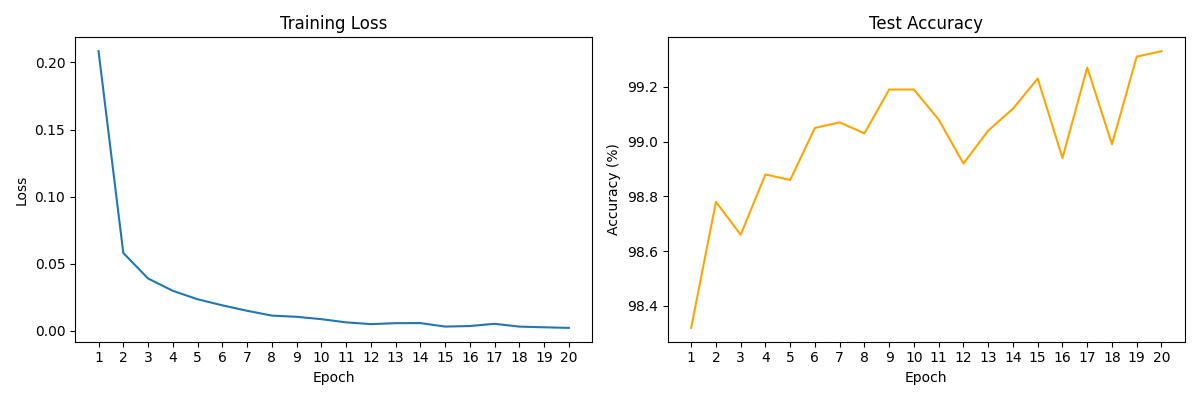
\includegraphics[width=0.96\linewidth]{../Figure/train_log.png}
		\caption{训练损失与测试准确率变化曲线}
	\end{figure}

	从实验结果来看，该模型能够较好地学习MNIST手写数字中的局部笔画特征。第一层卷积主要捕捉边缘和局部纹理，第二层卷积在下采样后的特征图上组合更抽象的笔画模式，最后通过全连接层完成类别判别。由于MNIST任务相对规整，即使没有额外的数据增强和复杂网络结构，两层卷积网络也能够达到较高准确率。

	\section{总结}
	本次实验基于PyTorch完成了MNIST手写数字识别任务，主要工作包括数据集加载与划分、CNN模型搭建、损失函数和优化器设置、训练日志记录、模型保存以及结果可视化。最终模型在测试集上取得99.33\%的准确率，满足实验指导书中测试集准确率达到98\%及以上的要求。后续如果继续改进，可以考虑固定随机种子以增强结果可复现性，在输入端加入标准化处理，或进一步补充混淆矩阵来分析各个数字类别之间的错误模式。

\end{document}
